% ============================================================================
% Results
% ============================================================================

\todo{ALL RESULTS IN THIS SECTION ARE PLACEHOLDERS.
Replace every \todo{} with measured values before submission.}

\subsection{Calibration and Static Accuracy}

Table~\ref{tab:ant_delays} (Section~\ref{sec:calibration}) lists per-board
antenna delays after Tier-1 calibration.
Uncalibrated mean range bias: \todo{X}\,mm.
After Tier-1: \todo{Y}\,mm.
After Tier-2 spatial map: \todo{Z}\,mm at held-out positions.

\todo{Insert Table: per-position static RMSE. Insert CDF figure.}

Table~\ref{tab:static_accuracy} summarises 2D static errors.

\begin{table}[h]
  \centering
  \caption{Static 2D position accuracy.}
  \label{tab:static_accuracy}
  \begin{tabular}{lcc}
    \toprule
    Configuration & Mean RMSE (cm) & $\epsilon_{90}$ (cm) \\
    \midrule
    No calibration & \todo{} & \todo{} \\
    + Tier-1       & \todo{} & \todo{} \\
    + Tier-2 map   & \todo{} & \todo{} \\
    + EKF (full)   & \todo{} & \todo{} \\
    \bottomrule
  \end{tabular}
\end{table}

\subsection{NLOS Mitigation}

Fig.~\ref{fig:nlos_gap} shows the NLOS gap distribution under LOS and
obstructed conditions.
\todo{Replace synthetic histogram with hardware data.}

With the obstructed anchor weighted ($w_i \approx \todo{w}$), position RMSE
reduced from \todo{X}\,cm to \todo{Y}\,cm.
\todo{Show trajectory with/without NLOS weighting and RMSE table comparing:
unweighted, weighted, and hard-rejected.}

\subsection{Sweep Rate and Multi-Tag Operation}

\todo{Figure: measured sweep rate (Hz) vs.\ $N$ anchors.
Theoretical: $f = 1/(N \times 25\,\text{ms})$.
Measured at $N = 3, 4, 5$.}

\todo{2-tag experiment: accuracy per tag during simultaneous operation;
show accuracy degradation vs.\ single-tag baseline is negligible.}

\subsection{Dynamic Tracking and Ablation}

\todo{Trajectory figure: estimated path vs.\ Kinect ground truth.
Report RMSE over full dynamic path.}

Table~\ref{tab:ablation} shows the per-component ablation.

\begin{table}[h]
  \centering
  \caption{Ablation --- contribution of each component to 2D RMSE.}
  \label{tab:ablation}
  \begin{tabular}{lccc}
    \toprule
    Configuration & Mean RMSE & $\epsilon_{90}$ & $\epsilon_{\max}$ \\
    \midrule
    No calibration    & \todo{} & \todo{} & \todo{} \\
    + Tier-1          & \todo{} & \todo{} & \todo{} \\
    + Tier-2 map      & \todo{} & \todo{} & \todo{} \\
    + NLOS weighting  & \todo{} & \todo{} & \todo{} \\
    + EKF (full system) & \todo{} & \todo{} & \todo{} \\
    \bottomrule
  \end{tabular}
\end{table}

\begin{figure}[h]
  \centering
  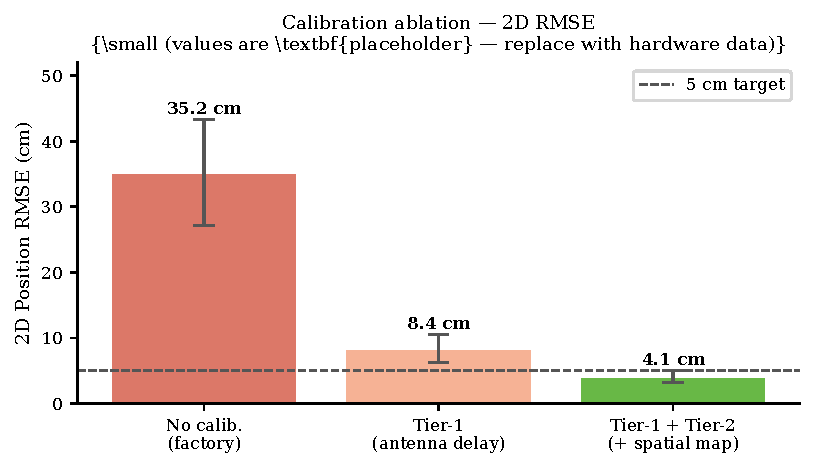
\includegraphics[width=0.90\columnwidth]{figures/calibration_effect.pdf}
  \caption{Calibration ablation: 2D position RMSE at each calibration tier.
  Values are \textbf{synthetic placeholders} --- replace with hardware data.}
  \label{fig:calib_effect}
\end{figure}
